\chapter{Shared Memory Architectures}
\label{ch:04/shared-memory-architectures}

Shared Memory Architectures are a type of MIMD architecture where all processors share the same memory space, and can access it directly. This is the most common architecture for multi-core processors (\textit{``multiprocessors''}).

They mirror the Von Neumann architecture, with multiple processors sharing the same memory space.

\section{Von Neumann Bottleneck}

\begin{definition}[von Neumann Bottleneck]
   The \textit{von Neumann bottleneck} is a limitation on throughput caused by the standard personal computer architecture. The term is named for John von Neumann, who is credited with developing the von Neumann architecture, in which programs and data are stored in the same memory. \ul{The bottleneck refers to the limited data transfer rate between a computer's CPU and memory compared to the amount of memory.}
\end{definition}

\begin{figure}[htbp]
   \centering
   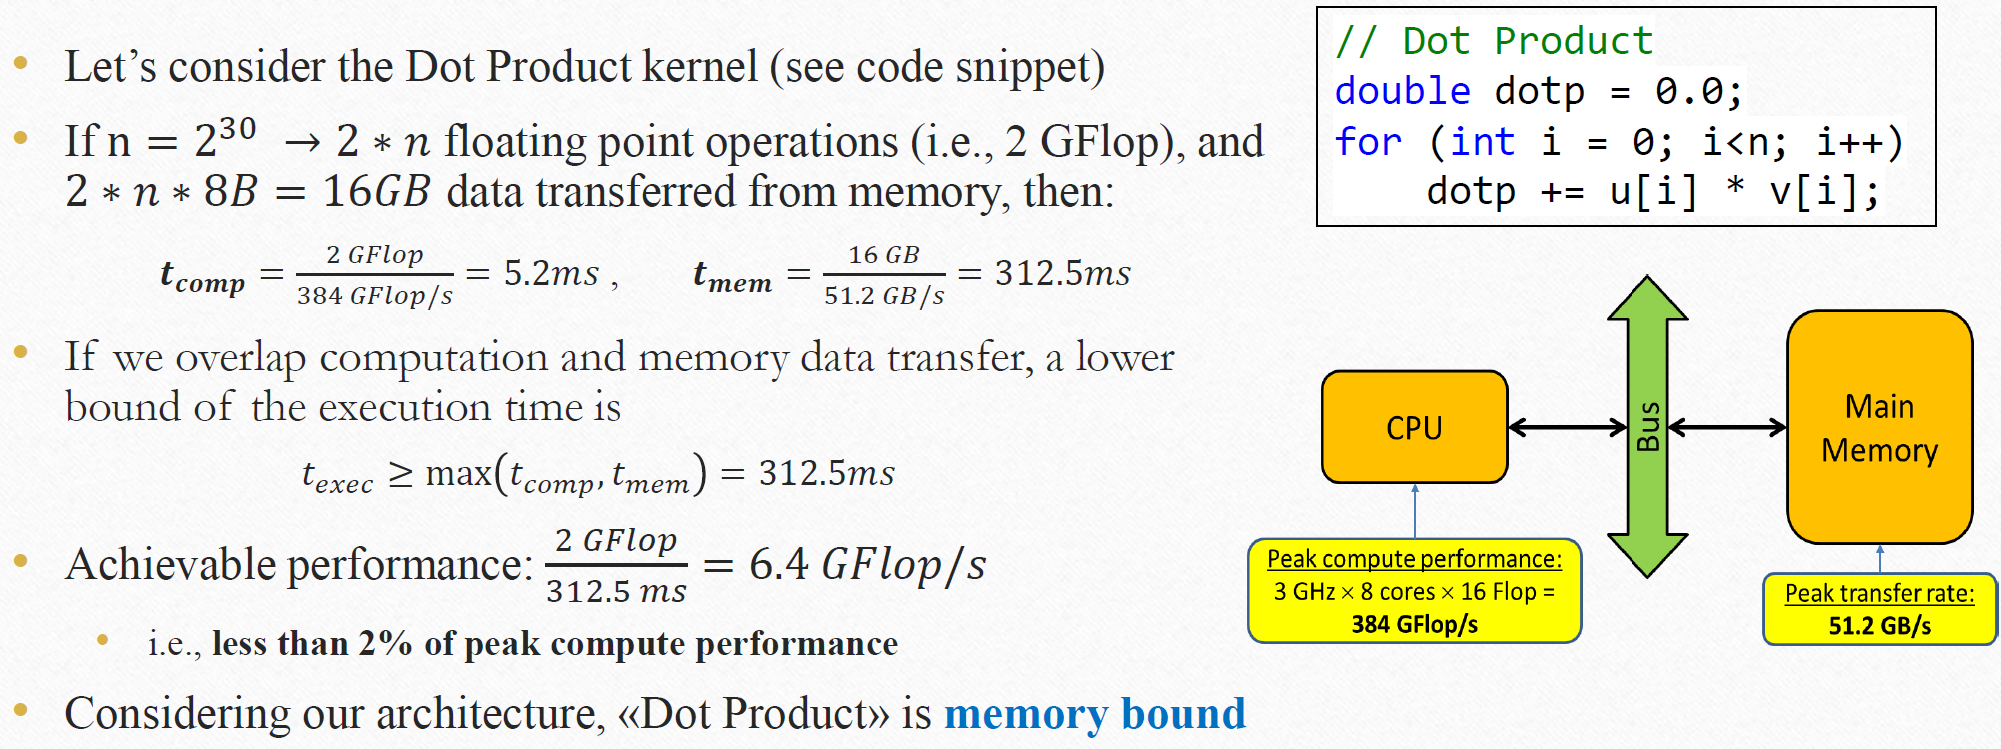
\includegraphics{images/04/neumann_example.png}
   \caption{von Neumann Bottleneck example}
   \label{fig:04/neumann_example}
\end{figure}

In the example in Figure \ref{fig:04/neumann_example}, the CPU is waiting for the data to be loaded from memory, which is a slow operation, leading to \ul{exploiting only the 2\% of the CPU capabilities.}

\subsection{Caches}

\begin{paracol}{2}
   Back in the day, the solution was to \textit{``move the data closer to the CPU''}, introducing \textbf{memory hierarchy} and \textbf{caches}.

   Usally, L1 and L2 are private to each core, while L3 is shared among all cores.
   \switchcolumn
   
   \begin{figure}[htbp]
      \centering
      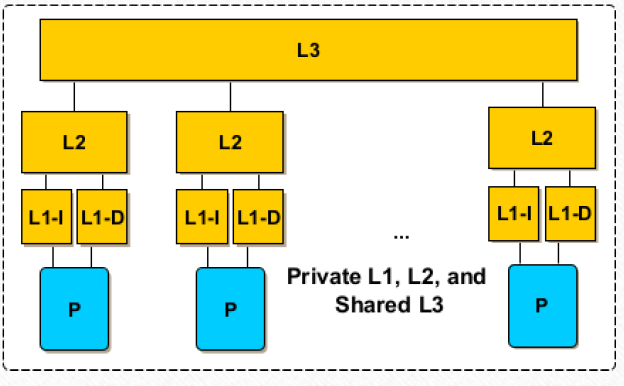
\includegraphics{images/04/caches_hierarchy.png}
      \caption{Caches hierarchy}
      \label{fig:04/caches_hierarchy}
   \end{figure}
\end{paracol}

If a matrix of the previous example in Fig. \ref{fig:04/neumann_example} is entirely stored in cache, then the achievable performance is \ul{223 GFLOPS, which is about 60\% of the peak power.}

If the matrices do not fit in the cache, the performance drops since we need to trap to the main memory to fetch missing data.\\
So, the problem shifts to understand how to exploit the cache to its fullest.

\section{Locality Principle}

The locality principle is the driving force that makes the cache work. Locality increases the probability of reusing data blocks that were previously moved from level $n$ to level $n-1$.
\begin{itemize}
   \item \textbf{Temporal Locality}: if a data is accessed, it is likely to be accessed again soon.
   \note{Cache mapping strategy (Direct/associative) and the replacement policy (LRU, FIFO, Random etc.) are crucial to exploit temporal locality.}
   \item \textbf{Spatial Locality}: if a data is accessed, it is likely that nearby data will be accessed soon.
\end{itemize}

\subsection{Measuring CPU time with caches}
\begin{equation}
   CPU_{time} = ClockCycles \cdot ClockCycleTime = IC \cdot ClockCycleTime
\end{equation}
\begin{itemize}
   \item IC: Instruction Count (number of instructions executed)
   \begin{itemize}
      \item $IC = IC_{CPU} + IC_{MEM}$
   \end{itemize}
   \item CPI: Cycles Per Instruction
   \begin{itemize}
      \item $CPI = \dfrac{ClockCycles}{IC}$
      \item $CPI = \dfrac{IC_{CPU}}{IC} \cdot CPI_{CPU} + \dfrac{IC_{MEM}}{IC} \cdot CPI_{MEM}$ where $CPI_{CPU}$ are the average cycles per ALU instruction and $CPI_{MEM}$ are the average cycles per memory instruction.
      \item Considering that each memory instruction may generate a cache hit or miss with a given probability, and naming $HitRate$ the probability of a cache hit, we can write 
      \begin{equation}
         CPI_{MEM} = HitRate \cdot CPI_{MEM - Hit} + (1-HitRate) \cdot CPI_{MEM - Miss}
      \end{equation}
   \end{itemize}
\end{itemize} 

\subsection{Cache Algorithms}
\begin{enumerate}
   \item \textit{What do we load from main memory?}
   \item \textit{Where do we store it in the cache?}
   \item \textit{Cache is full, what should we evict?}
\end{enumerate}

\note{At the beginning of the second half of the $4^{th}$ lecture, the professor displays how to VPN in the unipi and then ssh to the servers.}

\subsection{Cache mapping and eviction strategies}
\begin{itemize}
   \item \textbf{Direct-mapped} cache: each memory block can be placed in only one cache line.
   \item \textbf{n-way} set associative cache: each memory block can be placed in $n$ cache lines.
   \item \textbf{Least Recently Used} (LRU) cache: the block that has been accessed the least recently is evicted.
\end{itemize}

\framedt{Transposing Matrices}{
   Suppose you have to multiply matrix A and B. If you access A as rows, you'll access B as columns.\\
   Since matrices are stored in row-major order, you won't exploit spatial locality on B, and for each element of A you'll have a cache miss on B, creating the need to evict a line and load another one in cache.\\
   \textbf{Transposing} B would solve the problem, since you would access B as rows, exploiting spatial locality.

   Prof. Torquati displayed that transposing and then multiplying the matrices would lead to a 2x speedup.
   \note{17s vs 37s}
}

\subsection{Cache Write Policies}
Data in cache may be inconsistent with the value in memory, leading to the need to write back the data to memory. There are two policies:
\begin{itemize}
   \item \textbf{Write-through}: data is written to both cache and memory. It is simple but slow.
   \item \textbf{Write-back}: data is written only to the cache, and then to memory when the block is evicted. It is faster but more complex.
   \begin{itemize}
      \item Caches mark data in the cache as dirty (Dirty bit)
      \item When a dirty line is evicted, it is written in main memory
      \item A store write buffer is generally used to reduce the cost of cache writes
   \end{itemize}
\end{itemize}

\subsection{Cache Coherence}
\begin{paracol}{2}
   With private caches per core, it is possible to have several copies of shared data in distinct caches, each cache stores a different value for a single address location.
   
   \begin{definition}[Cache incosistency]
      Two caches store different values for the same variable.
   \end{definition}
   
   \switchcolumn

   \begin{figure}[htbp]
      \centering
      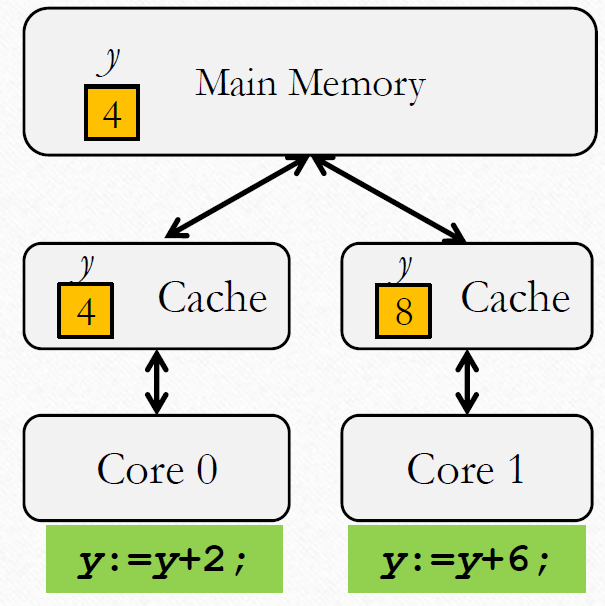
\includegraphics{images/04/cache_coherence.png}
      \caption{Cache incosistency problem}
      \label{fig:04/cache_coherence}
   \end{figure}

\end{paracol}

Hardware firmware automatically solves this problem, but it is important to know that it exists.
The algorithms responsible for this are called \textbf{cache coherence protocols}, a famous one is the \textbf{MESI} protocol, but we ain't going to study it.
Note however that \ul{the cache coherence protocol granularity is the \textit{cache line}, not the \textit{single variable}.}
   
\section{Suggested readings}
\begin{itemize}
   \item
      Chapter 3.1 of the Parallel Programming Concept and Practice book
   \item
      Cache-coherence protocols: ``A Primer on Memory Consistency and Cache Coherence'' Daniel J. Sorin, Mark D. Hill, and David A. Wood
\end{itemize}

\section{Advanced Processors and Technologies}
\subsection{Superscalar CPUs}
Superscalar CPUs are designed to execute multiple instructions from a single process/thread simultaneously to improve performance and CPU utilization

The processor fetches multiple instructions concurrently in a single clock cycle and executes them out-of-order, exploiting instruction-level parallelism, Results are then re-ordered to ensure they are written back to the register file or memory in the correct program order

However, in sequential programs, the number of instructions that are independent are small thus, the exploited parallelism is low.
To overcome this limitation, \textbf{SMT} (\textit{Simultaneous Multi-Threading}) has been added in superscalar processors to execute multiple instructions from multiple threads of control simultaneously.
\note{Hyperthreading is Intel's implementation of SMT}

\subsection{HW Multithreading}
HW multithreading enablesa single core to execute multiple threads concurrently.
There are two main types of HW multithreading:
\begin{itemize}
   \item \textbf{Fine-grained multithreading}: the processor switches between threads at each cycle (instruction level).
   \item \textbf{Coarse-grained multithreading}: the processor switches between threads only when the thread in execution causes a stall.
\end{itemize}

Each thread has its own set of registers and program counter; the processor maintains the context of each thread to quickly switch between them.
However, they share the same cache and execution units.
For the OS, each context is seen as a logical core.

\section{Programming Shared Memory Systems}
\subsection{Threads are the way to go}

Thread creation is more lightweight and faster (from 3x to 5x) than process creation\footnote{A \texttt{fork} system call requires copying (\texttt{memcpy}) more data, e.g. page table}, and threads share the same memory space, so they can communicate easily.
Creating a thread takes $\mathcal{O}(10^4)$ cycles in C/C++.

\subsection{Data-race}
\begin{definition}
   [Data Race] Scenario that occurs when two threads access a shared variable simultaneously and at least one of the accesses is a write, and the accesses are not guarded by a synchronization operation.   
\end{definition}
\begin{paracol}{2}
   DRs produce non-deterministic results, and are hard to debug, since they depend on the thread scheduling. To avoid this issue, we may use \textit{mutexes, condition variables, semaphores, atomic operations, etc.}
   
   \note{We will discuss all four, except \textit{semaphores}, which are more common in processes synchronization.}
   
   \switchcolumn

   \begin{figure}[htbp]
      \centering
      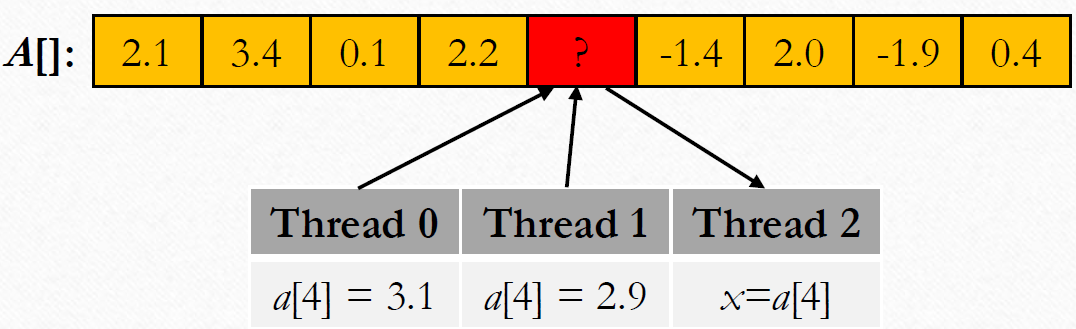
\includegraphics{images/04/data_race.png}
      \caption{Data Race example}
      \label{fig:04/data_race}
   \end{figure}

\end{paracol}

\subsection{False Sharing}
Caches are organized in cache lines, and cache coherence is managed at the cache line granularity. 
\begin{definition}
   [False Sharing] Scenario that occurs when two threads access different variables that reside on the same cache line. The cache coherence protocol will invalidate the cache line, so actually the two threads won't share anything.
\end{definition}


\begin{figure}[htbp]
   \centering
   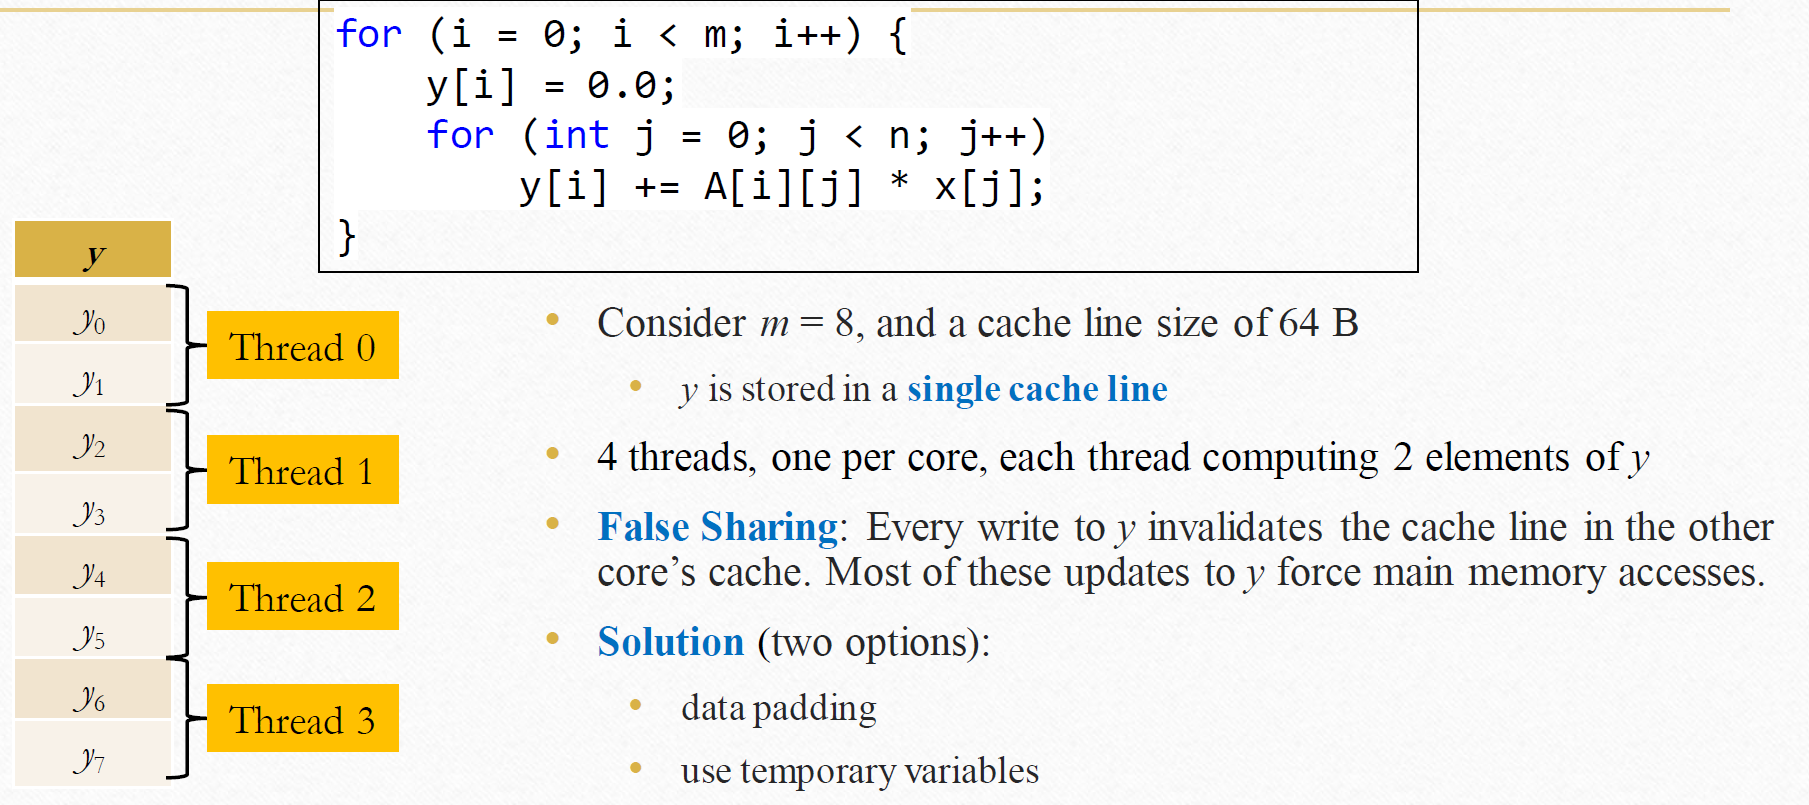
\includegraphics{images/04/false_sharing.png}
   \caption{False Sharing slide}
   Different threads access different variables which however reside on the same cache line.
   \label{fig:04/false_sharing}
\end{figure}
When False Sharing occurs, the performance of the system is degraded, since the cache line is invalidated and the cache coherence protocol keeps the cache line consistent among all copies.

Looking at Fig. \ref{fig:04/false_sharing}, suppose that $T_1$ accesses $y_2$:
the entire $y$ cache line is ---marked as?--- \textbf{invalidated}, so when $T_1$ accesses $y_1$, it will have a cache miss, and the cache line will be \st{reloaded from memory} ``moved from one core to another''\footnotemark[2]


\footnotetext[2]{Prof. Torquati said this, not sure if saying it gets ``reloaded from mem'' is correct}.

\newpage

\subsubsection{Padding}

\begin{figure}[htbp]
   \centering
   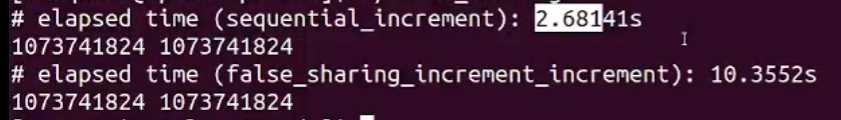
\includegraphics{images/04/false_sharing_demo.png}
   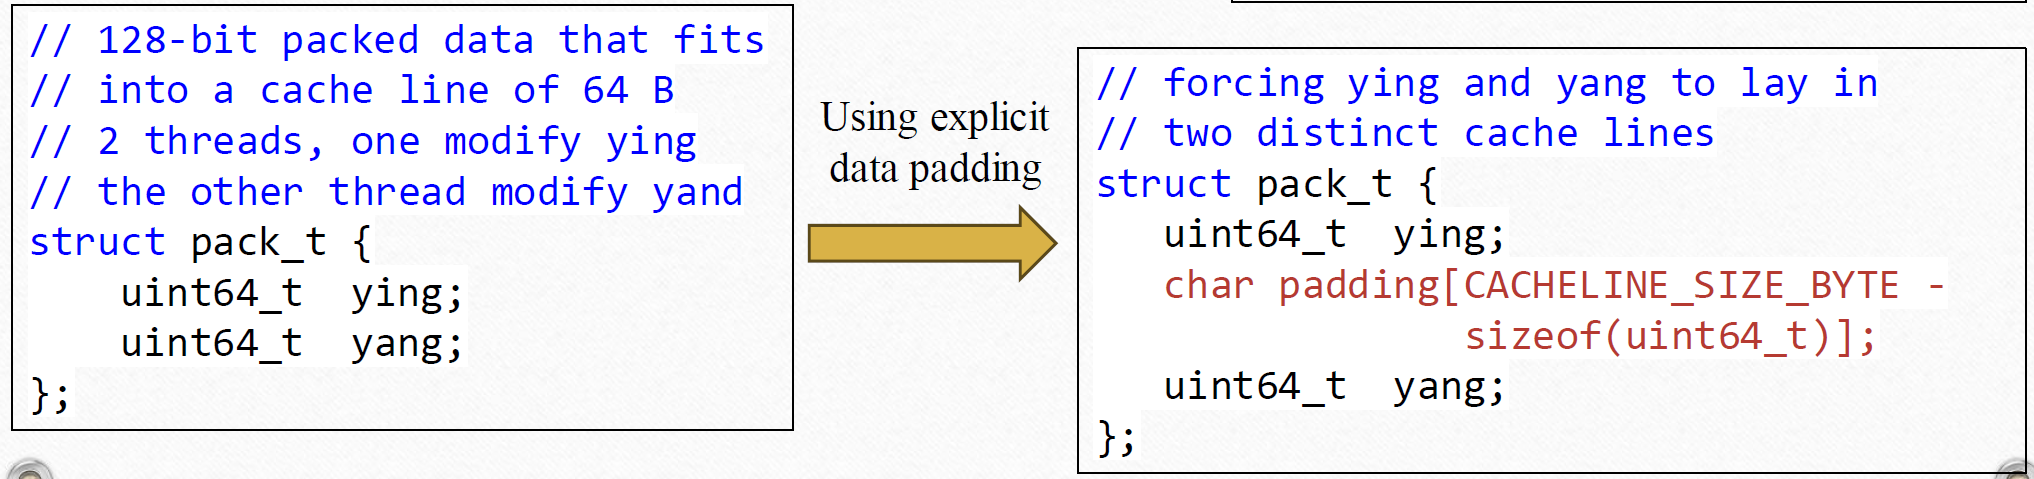
\includegraphics{images/04/false_sharing_program.png}
   \caption{False Sharing demo exec demo}
   \label{fig:04/false_sharing_demo}
   Prof. Torquati displayed that the exec time of a dummy program which increments two distinct variables in a struct went from 2.6s to 10.3s, when going from sequential to parallel execution. The overhead is due to false sharing.
\end{figure}

Fig. \ref{fig:04/false_sharing_demo} also displays a possible solution to the problem: \textbf{padding} the struct with a dummy variable, so that the two variables are placed on different cache lines. Even though looks a bit hardcoded, it works indeed!
Exec time, went from 2.6s to 2.9s, basically the same time, since the two variables are now on different cache lines; there is only some overhead due to the threads creation.

\framedt{How can i understand if false sharing is happening in a complex program?}{Test.}

\subsubsection{Local variables}

\begin{paracol}{2}

   \colfill
   Actually the better solution would be to use \textbf{local variables}, since they are stored in registers, and each thread has its own stack, so there is no sharing at all.
   \colfill

   \switchcolumn
   
   \begin{figure}[htbp]
      \centering
      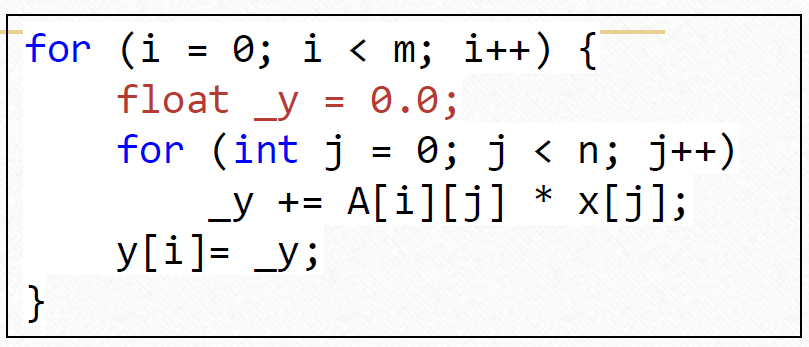
\includegraphics{images/04/false_sharing_local.png}
      \caption{Local variable stored in registers}
      \label{fig:false_sharing_local}
   \end{figure}
\end{paracol}
      

\framedt{Compiler optimization}{
   Modern compilers are able to optimize the code and avoid false sharing. If the example in Fig. \ref{fig:04/false_sharing_demo} is compiled with \texttt{g++ -O3} (instead of \texttt{-O0}), the exec time goes back to normal.

   However, it is not always possible to rely on the compiler, and in fact many times it does not work. So, it is better to pad the struct or use local variables, or avoid false sharing in general.
}
\newpage
\section{SIMD and Vectorization}
\textbf{SIMD} - \textit{Single Instruction, Multiple Data}. A parallel computing model that exploits data-level parallelism.
There are two limitations which must be kept in mind:
\begin{enumerate}
   \item ALUs are \textit{limited in number}, so the number of operations that can be executed in parallel is limited.
   \item All ALUs must execute the \textit{same instruction}.
\end{enumerate}

\begin{figure}[htbp]
   \centering
   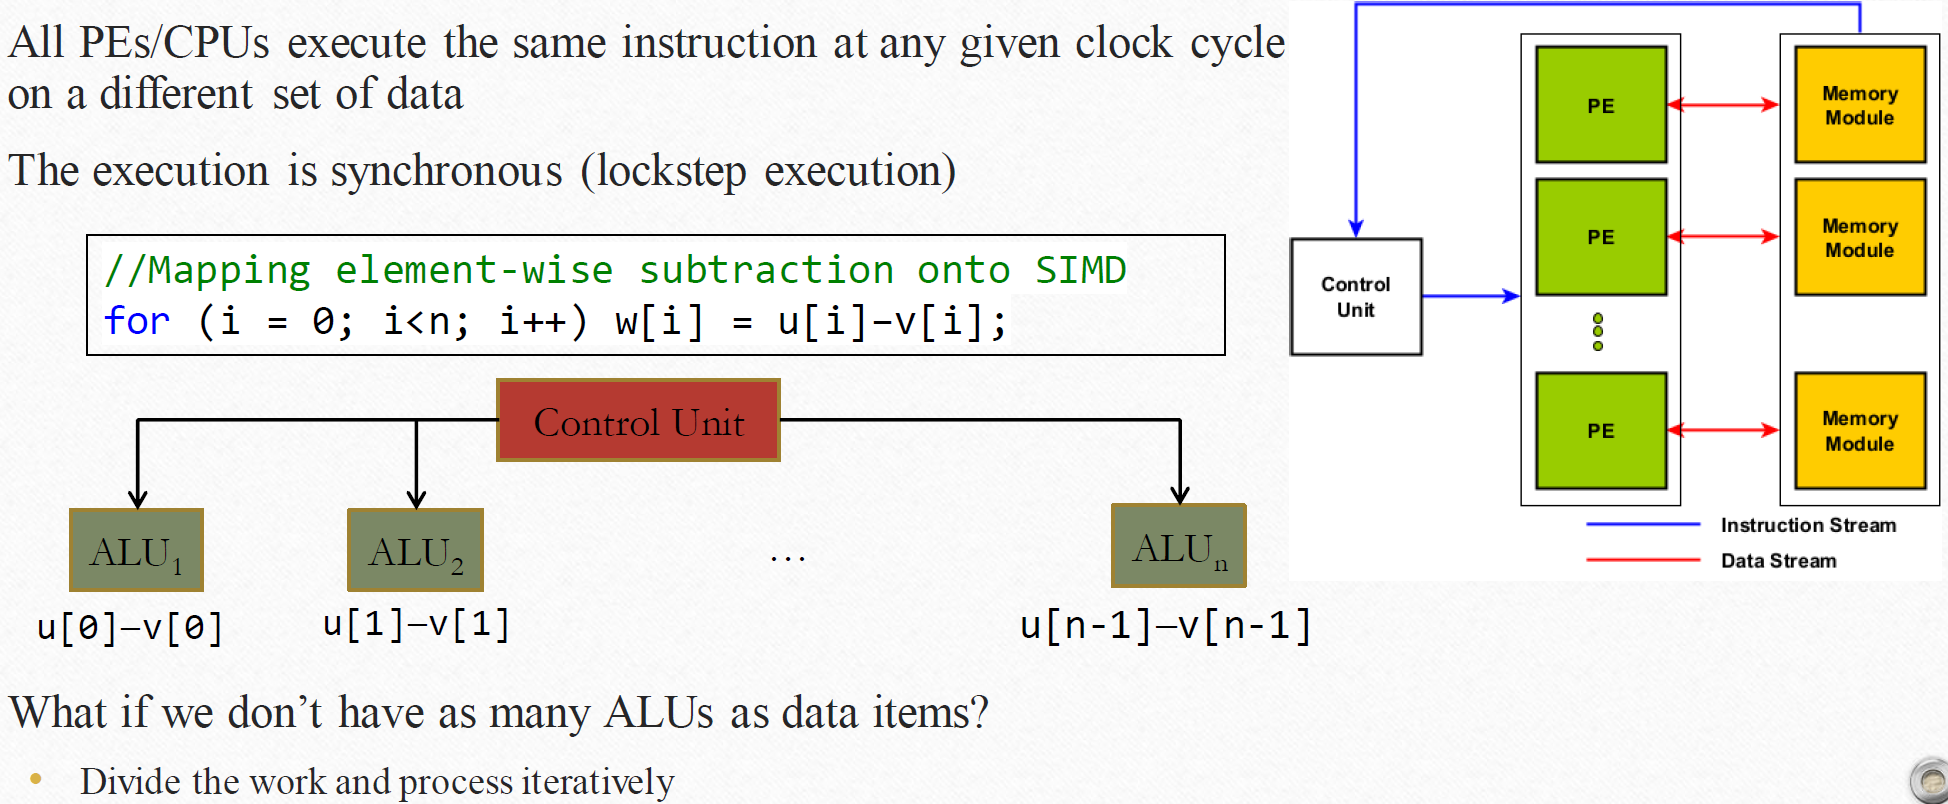
\includegraphics{images/04/SIMD.png}
   \caption{SIMD and ALUs}
   \label{fig:04/SIMD}
\end{figure}

\begin{figure}[htbp]
   \centering
   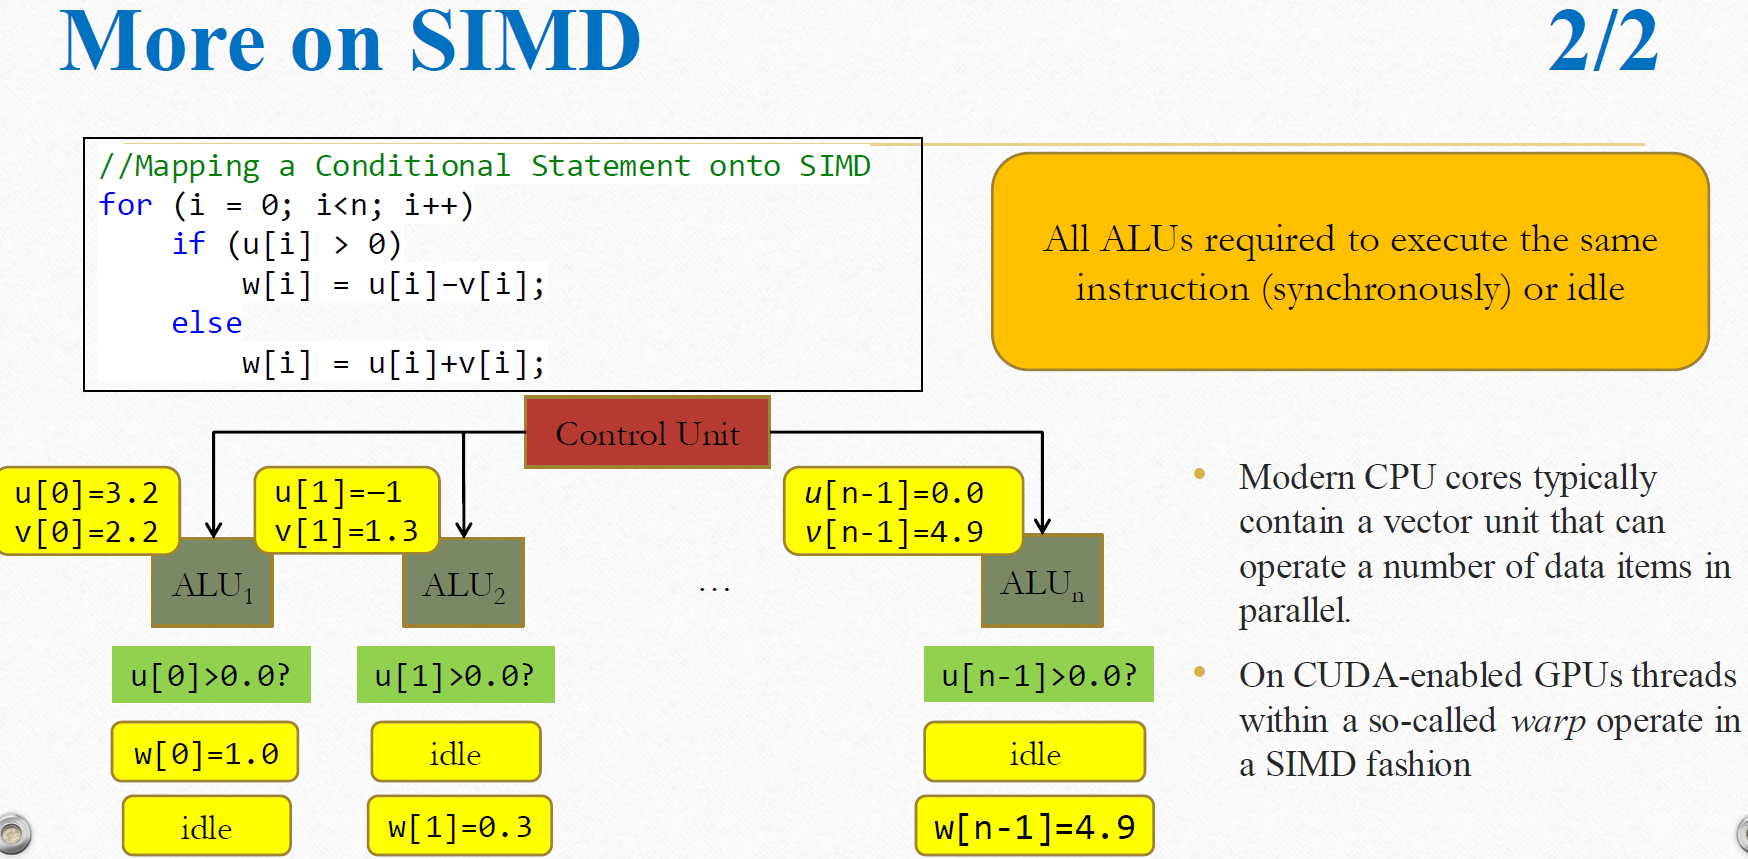
\includegraphics{images/04/SIMD2.png}
   \caption{Here the ALUs either execute an instruction ---another ALU is performing--- or stay \textbf{idle}.}
   \label{fig:04/SIMD2}
\end{figure}

\subsection{AVX registers}

\begin{lstlisting}[language=C,label={lst:04/avx},caption={Intrinsics}]
   //AVX-Programming with C/C++ Intrinsics
   __m256 a, b, c; // declare AVX registers
   ... // initialize a and b
   c = _mm256_add_ps(a, b); // c[0:8] = a[0:8] + b[0:8]
   // or c = _mm512_add_pd(a, b); c[0:8] = a[0:8] + b[0:8]
\end{lstlisting}

\textbf{Intrinsics} are assembly-coded functions that can be used in C/C++ to exploit SIMD parallelism. They are provide a light abstraction from assembly.
Exploiting intrinsics as in Lst. \ref{lst:04/avx} may lead to a 8x speedup, they are very powerful.

\begin{figure}[htbp]
   \centering
   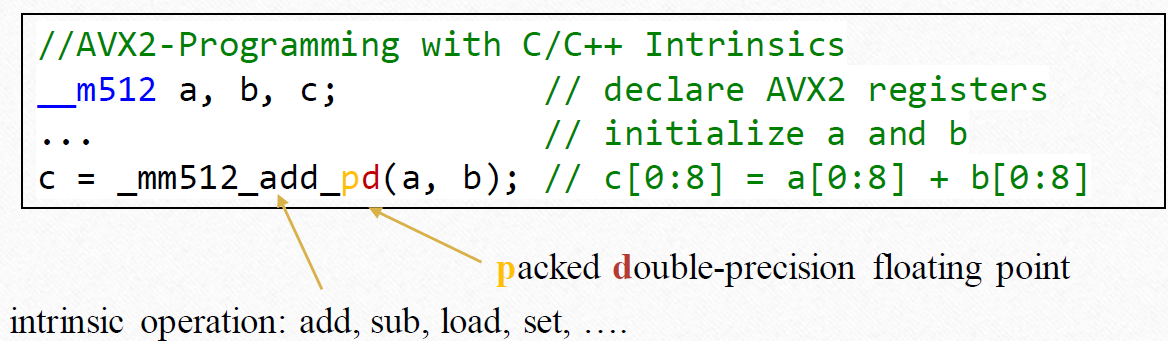
\includegraphics{images/04/intrinsics.png}
   \caption{Intrinsics explained}
   \label{fig:04/intrinsics}
\end{figure}